\chapter{Практическая часть}

На рисунках ниже представлена блок-схема алгоритма работы системного вызова open().

\begin{figure}[H]
    \centering
    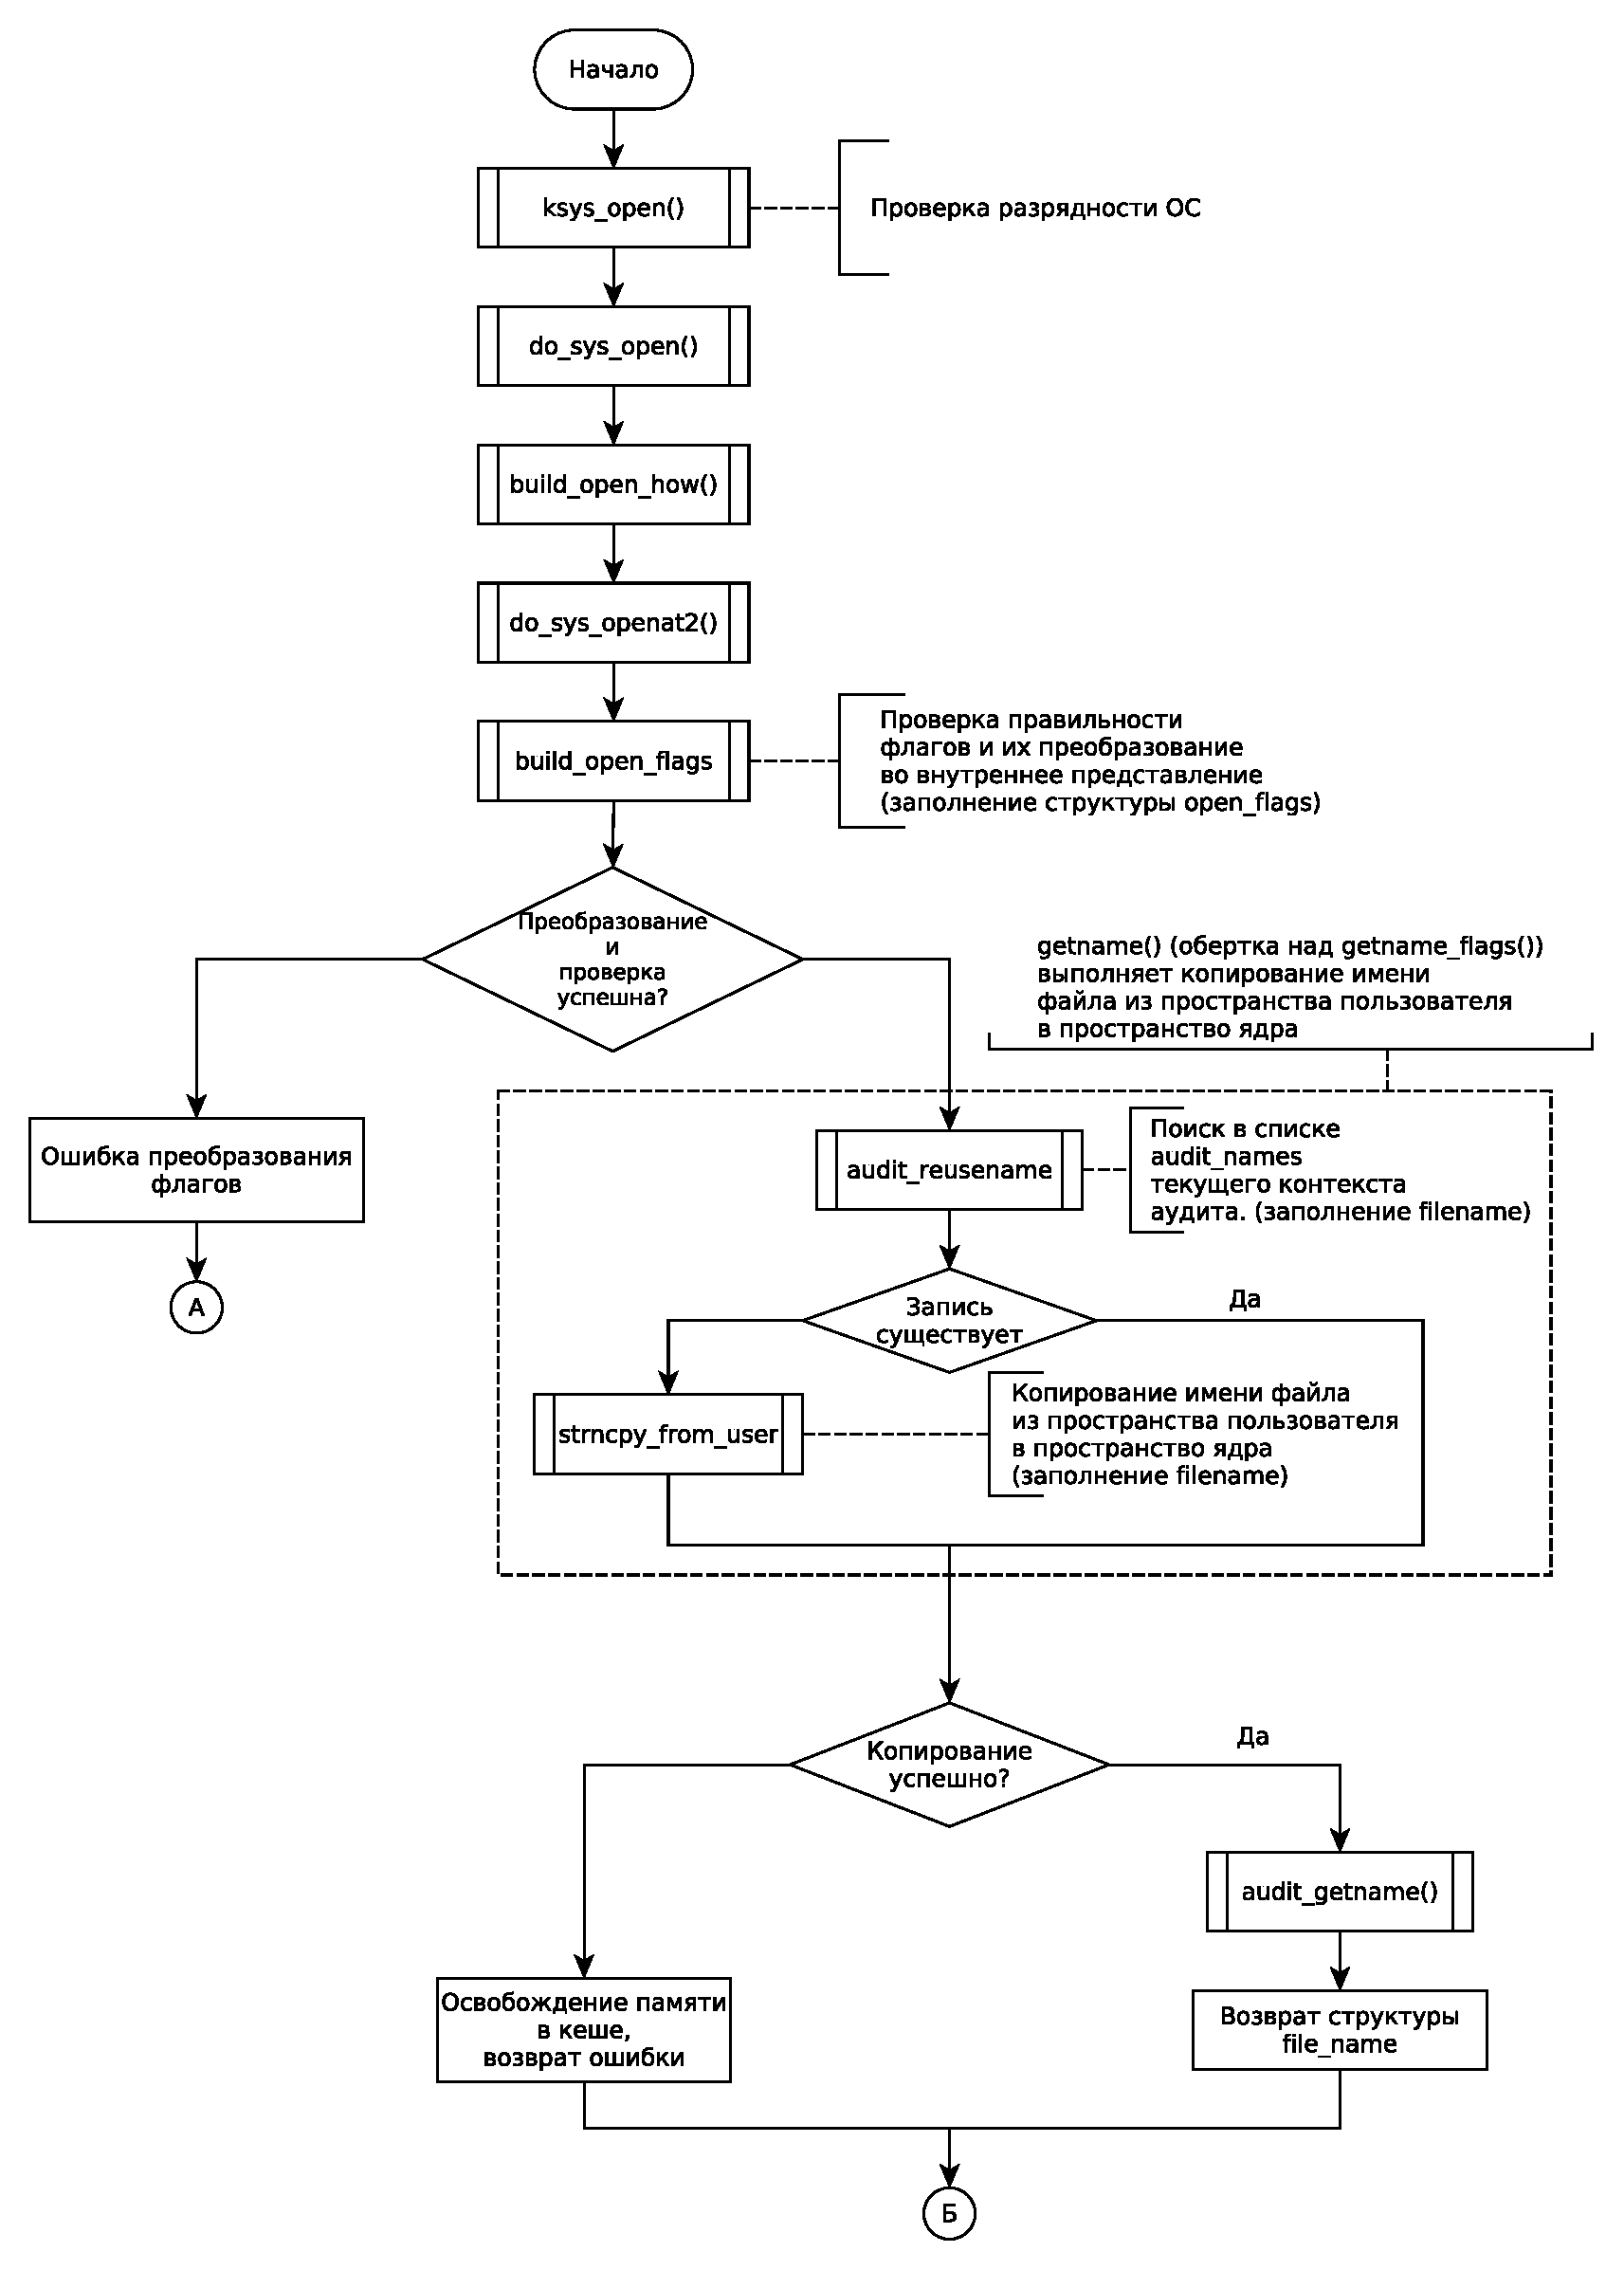
\includegraphics[scale=0.6]{data/newpdg/open_1.pdf}
    \caption{Блок-схема алгоритма open() (часть 1).}
\end{figure}

\begin{figure}[H]
    \centering
    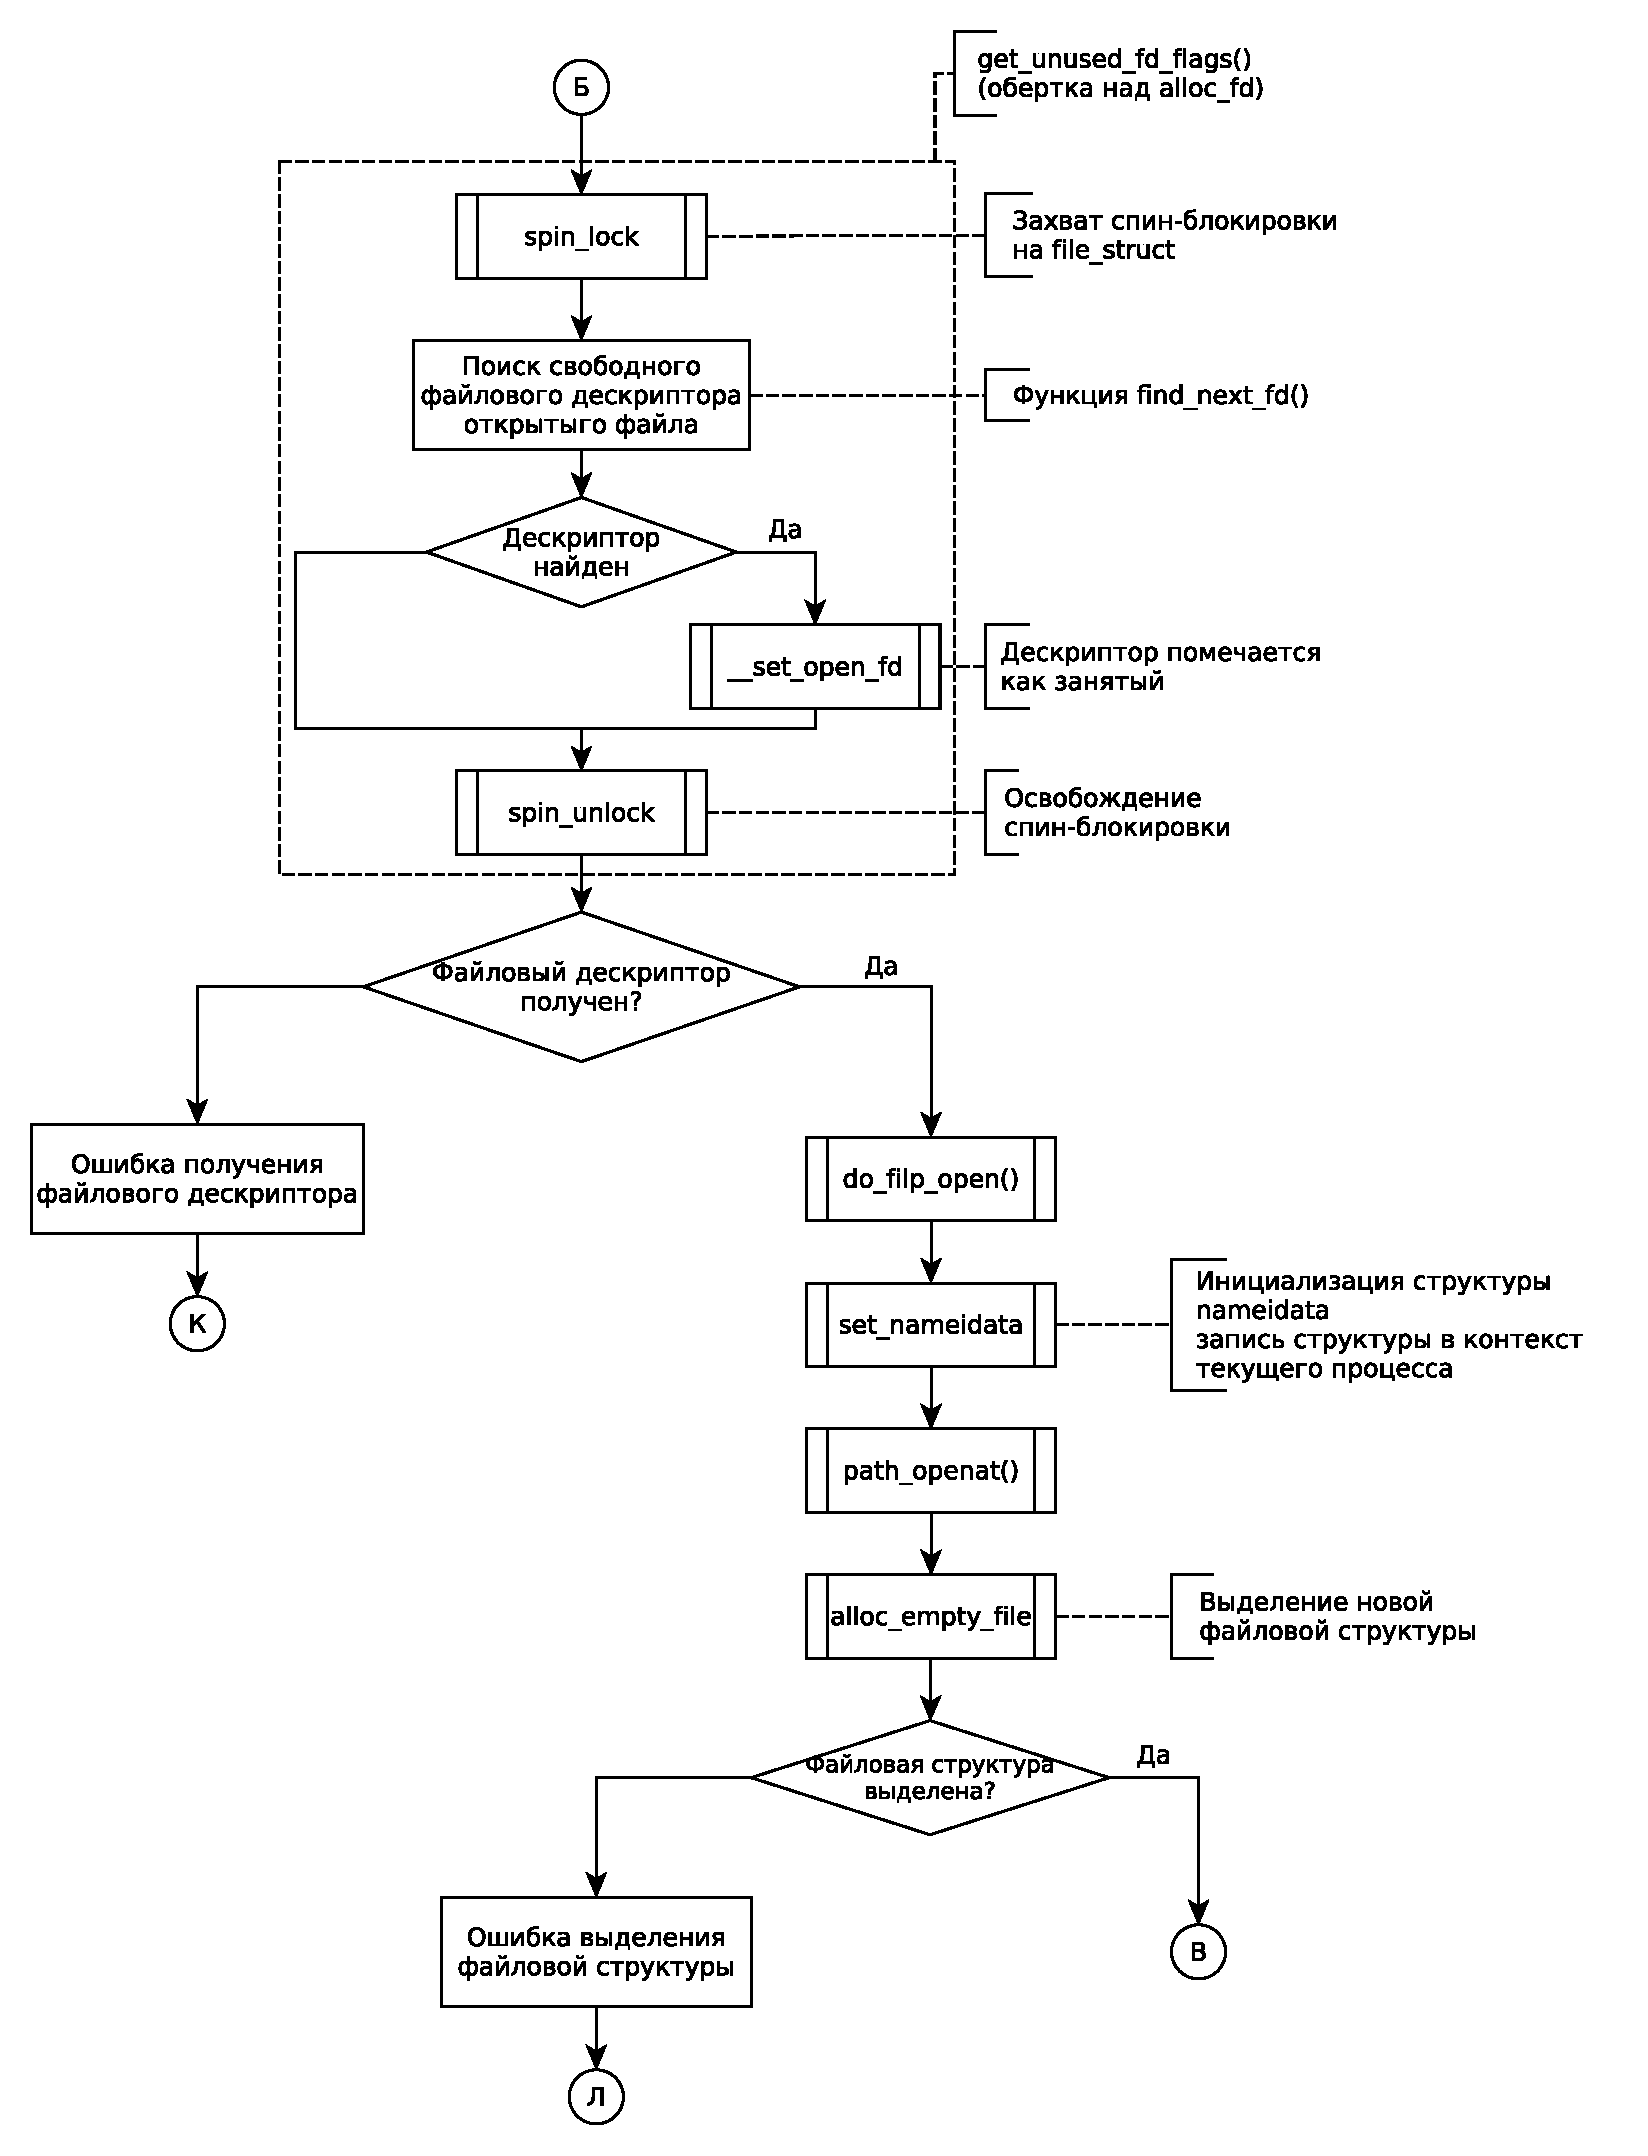
\includegraphics[scale=0.6]{data/newpdg/open_2rolaned.pdf}
    \caption{Блок-схема алгоритма open() (часть 2).}
\end{figure}

\begin{figure}[H]
    \centering
    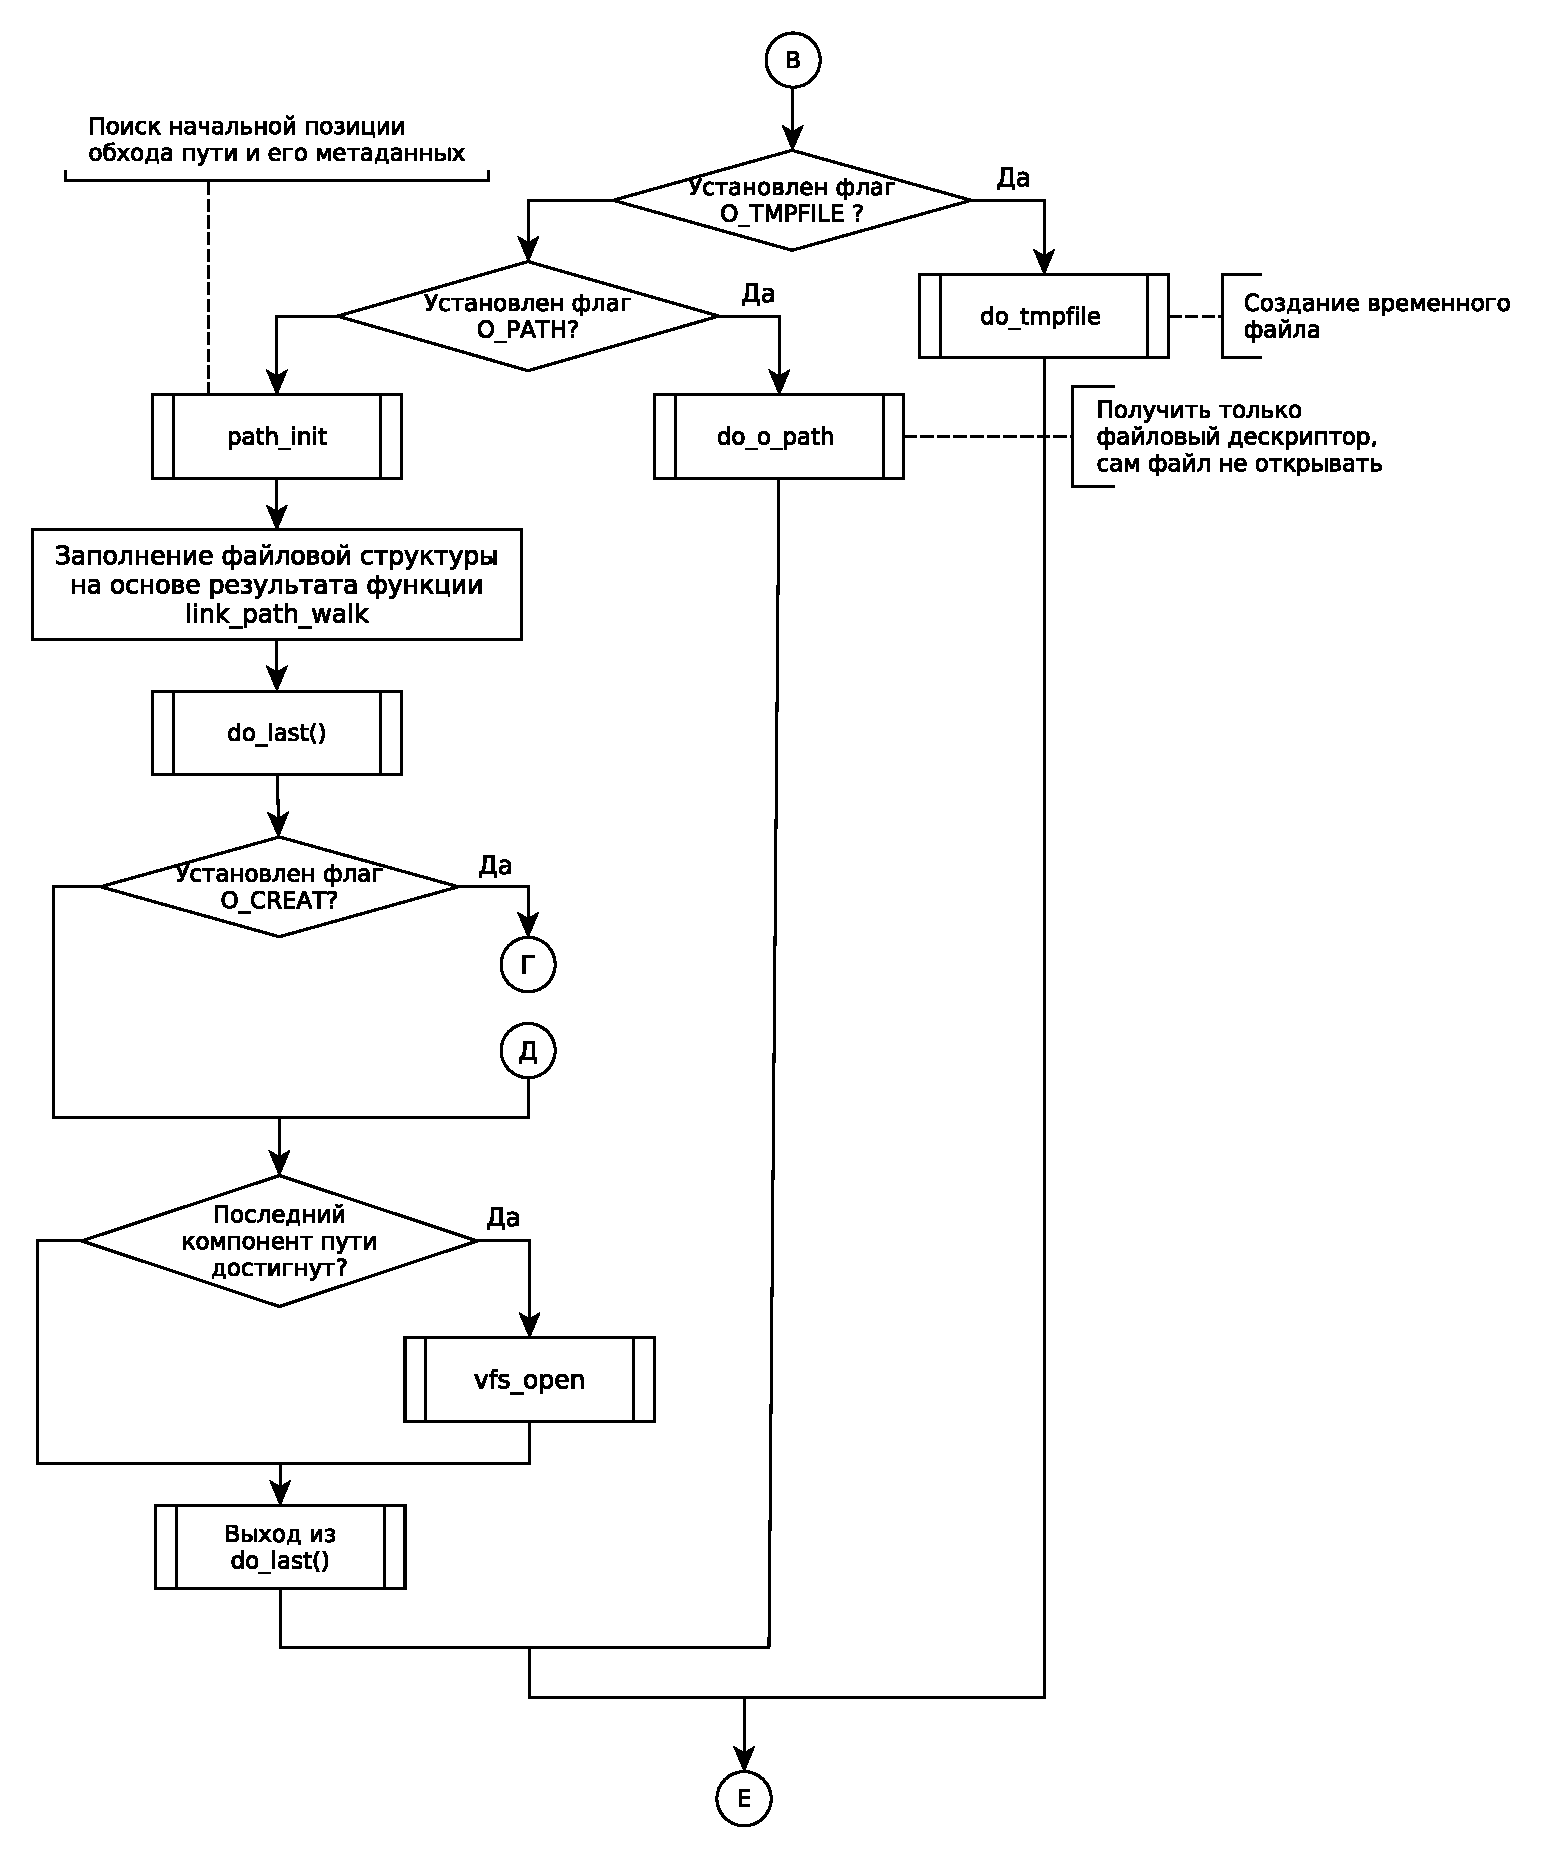
\includegraphics[scale=0.6]{data/newpdg/open_03_tryrolaned.pdf}
    \caption{Блок-схема алгоритма open() (часть 3).}
\end{figure}

\begin{figure}[H]
    \centering
    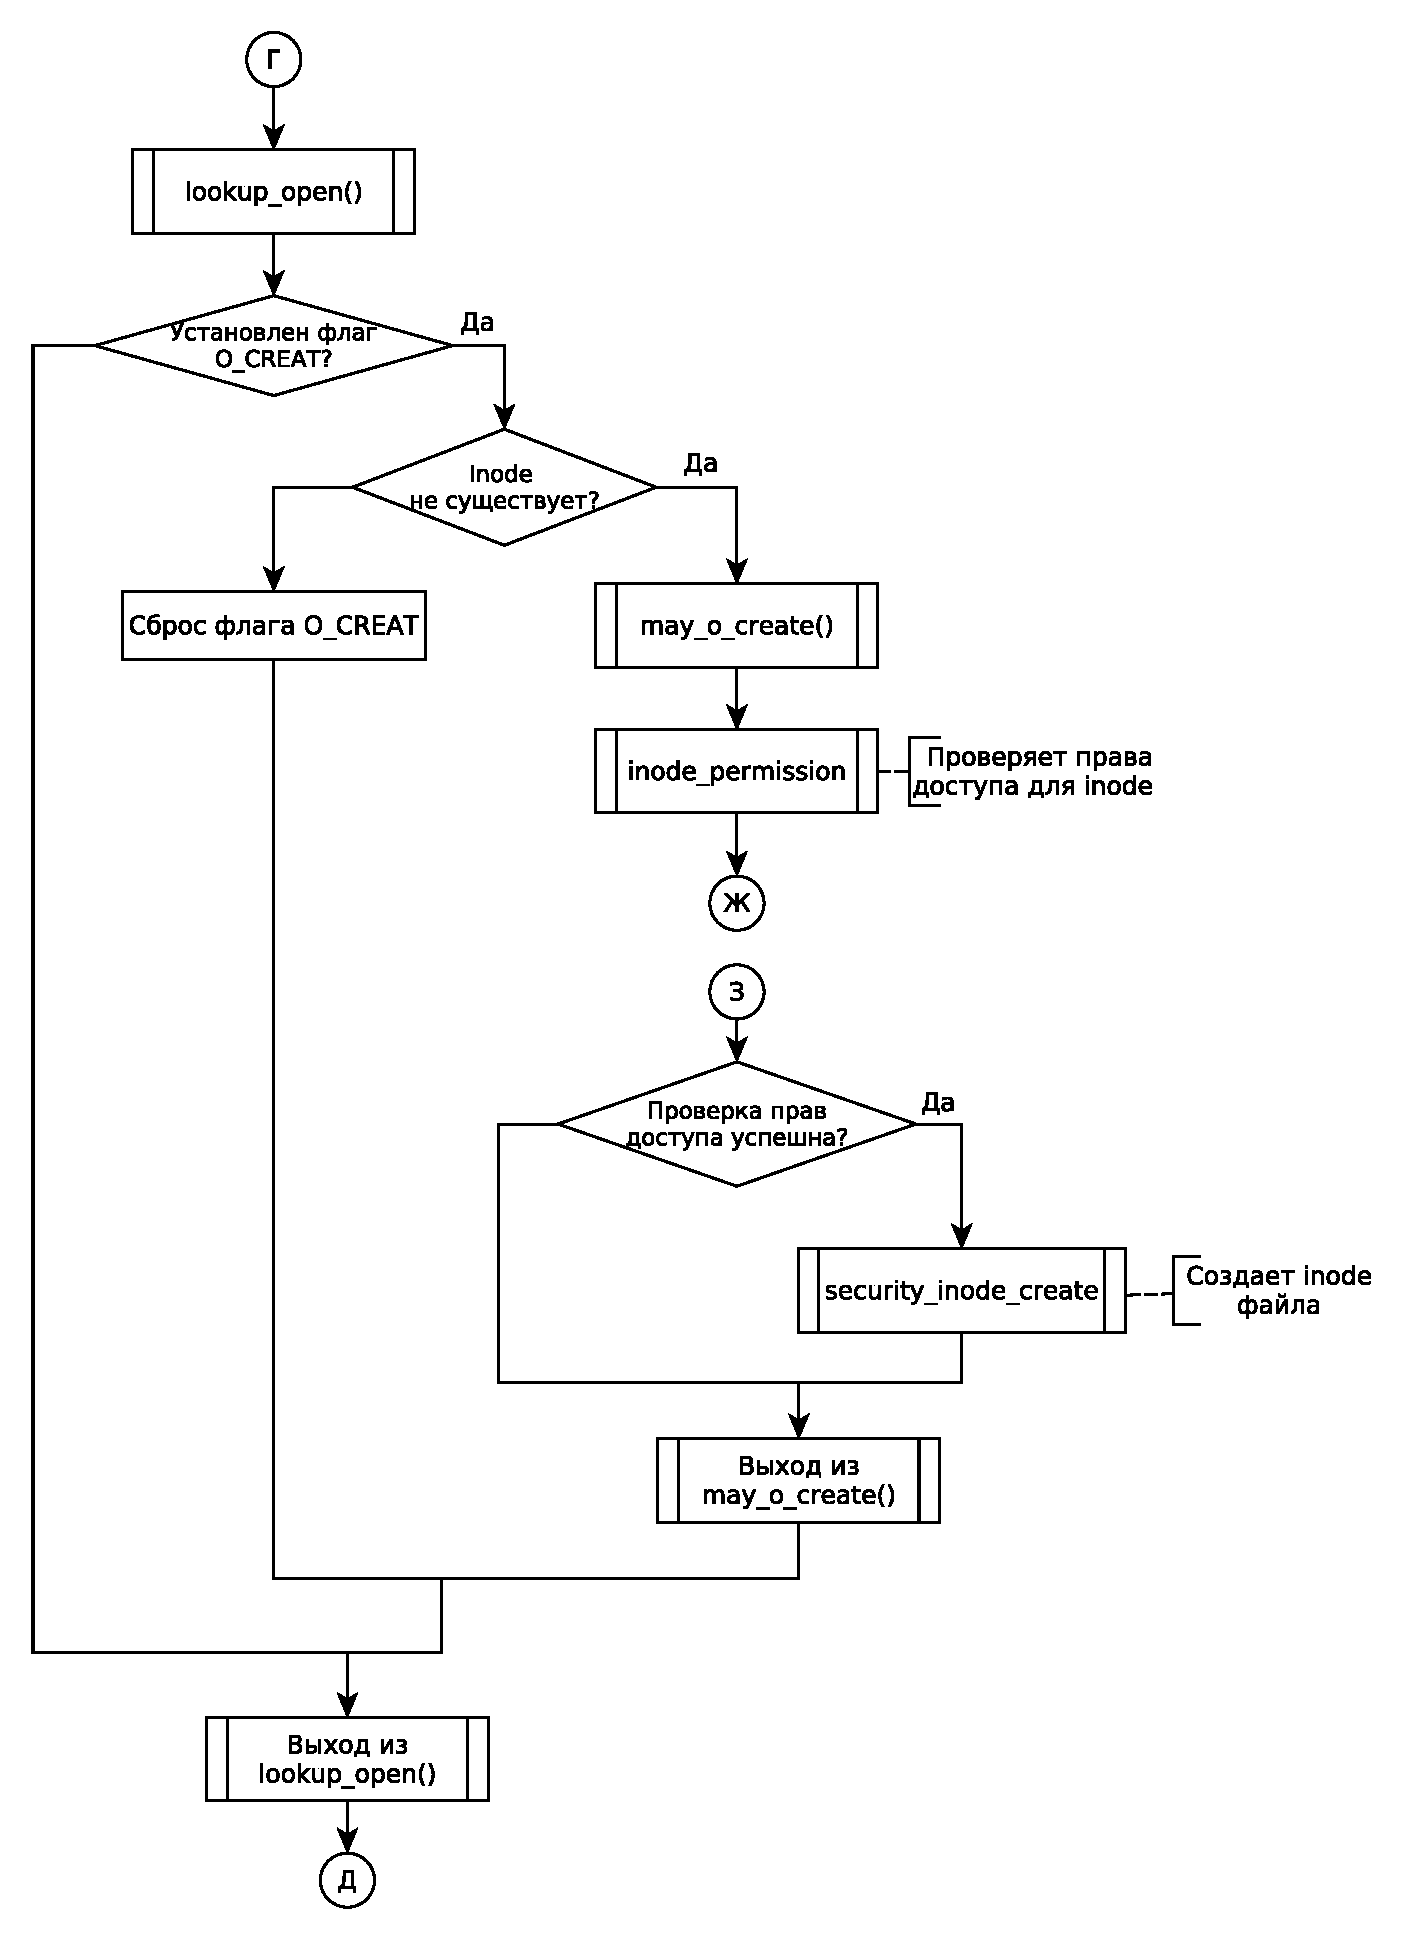
\includegraphics[scale=0.6]{data/newpdg/open_4_may_o_create.pdf}
    \caption{Блок-схема алгоритма open() (часть 4).}
\end{figure}

\begin{figure}[H]
    \centering
    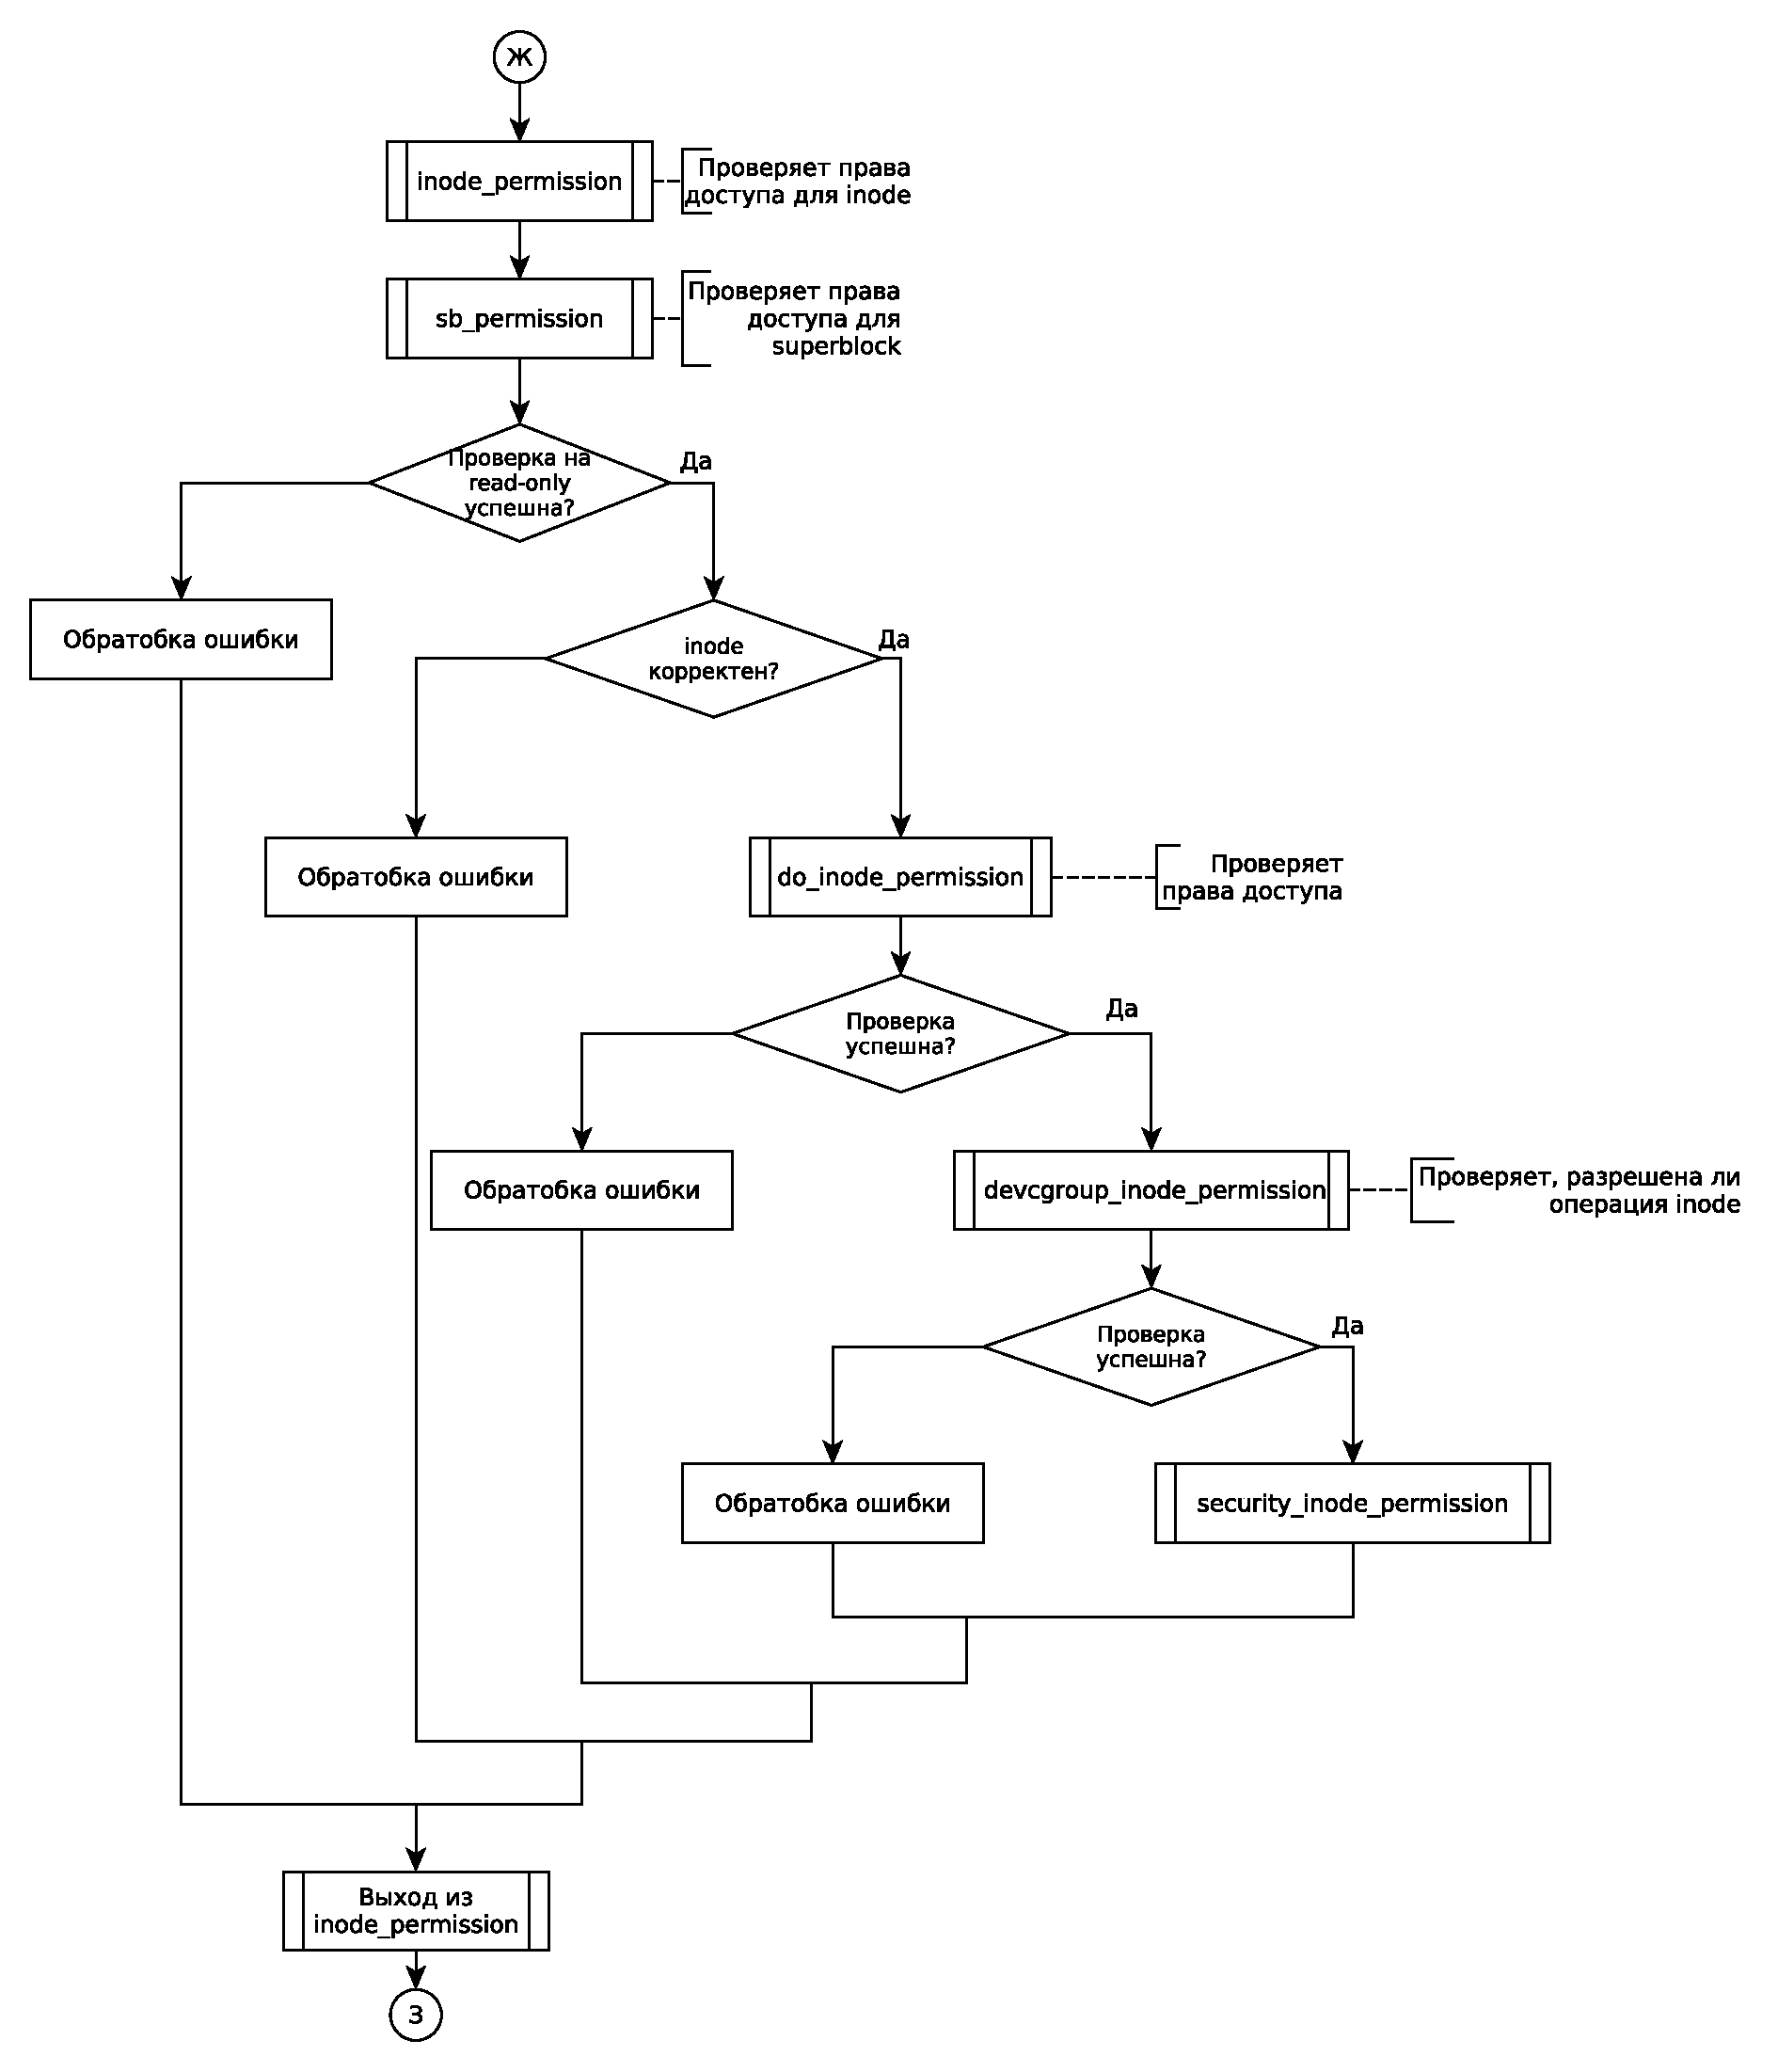
\includegraphics[scale=0.55]{data/newpdg/permissions.pdf}
    \caption{Блок-схема алгоритма open() (часть 5).}
\end{figure}

\begin{figure}[H]
    \centering
    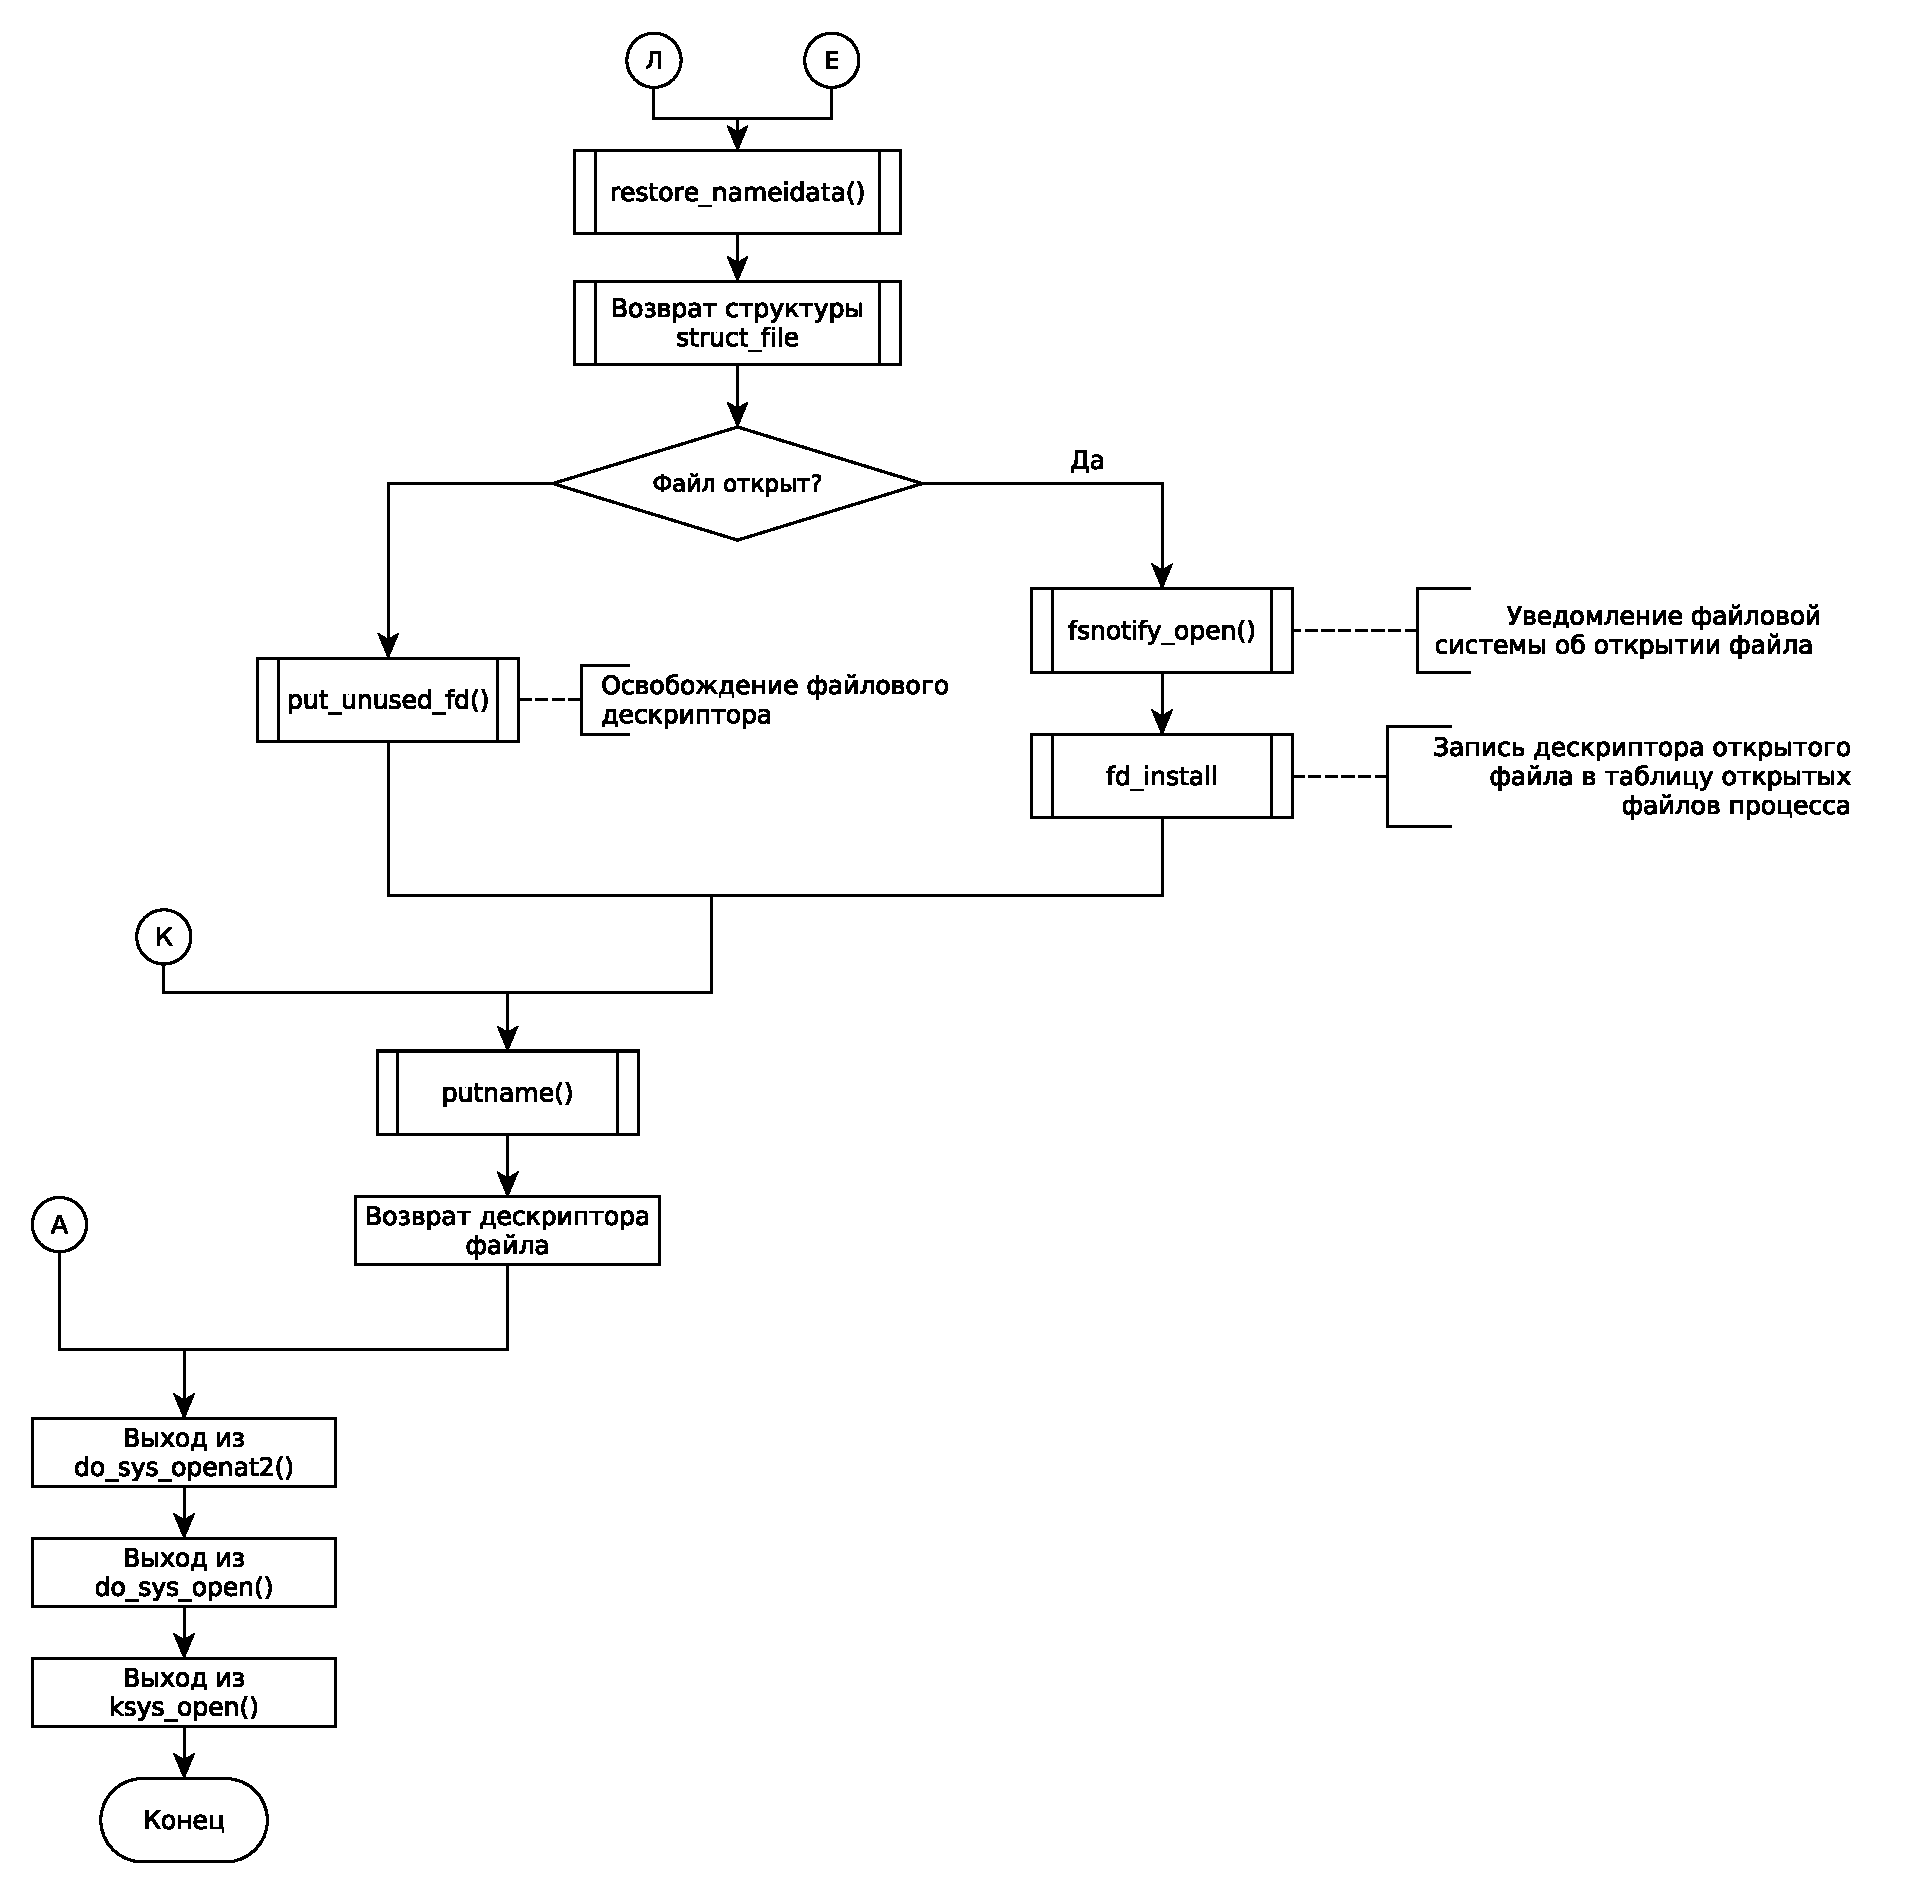
\includegraphics[scale=0.55]{data/newpdg/open_05.pdf}
    \caption{Блок-схема алгоритма open() (часть 6).}
\end{figure}
